\chapter{Kitaev model}

	\section{Model}

		Consider a spin-$\frac 1 2$ honeycomb lattice as shown of \autoref{fig:kitaevHoneycomb}. Separate it into two sublattices, even and odd. Links between vertices are divided into $x$, $y$ and $z$ one. The Hamiltonian is then written as
		\be \mc H = -J_x \sum_{x\text{-links}} \sigma_j^x \sigma_k^x - J_y \sum_{y\text{-links}} \sigma_j^y \sigma_k^y - J_z \sum_{z\text{-links}} \sigma_j^z \sigma_k^z \ee
		with Pauli matrices. Introduce a special notation
		\be K_{jk} = \begin{cases} \sigma_j^x \sigma_k^x & \text{if } (jk) \text{ is a $x$-link} \\ \sigma_j^x \sigma_k^y & \text{if } (jk) \text{ is a $y$-link} \\ \sigma_j^x \sigma_k^z & \text{if } (jk) \text{ is a $z$-link} \end{cases} \ee

		\begin{figure}[h!]
            \centering
            \includegraphics[scale=0.2]{graphs/kitaevHoneycomb.png}
            \caption{Representation of the Honeycomb lattice with the specific notation for the Kitaev model.}
            \label{fig:kitaevHoneycomb}
        \end{figure}

		Introduce also operators associated to lattice plaquettes $p$
		\be \begin{split} W_p &= \sigma_1^x \sigma_2^y \sigma_3^z \sigma_4^x \sigma_5^y \sigma_6^z \\ &= - \sigma_1^z \sigma_2^z \sigma_2^x \sigma_3^x \sigma_4^x \sigma_4^y \sigma_5^y \sigma_5^z \sigma_6^z \sigma_6^y \sigma_1^y \\ &= K_{12} K_{23} K_{34} K_{45} K_{56} K_{61} \end{split} \ee
		with labeling as in \autoref{fig:labelKitaevHCL}. It is obvious that
		\be [W_{p_1}, W_{p_2}] = 0 \quad \forall p_1 \neq p_2 \ee
		and the commutation with the Hamiltonian
		\be [\mc H, W_p] = 0 \quad \forall p \ee
		follow from the anticommutation relations of the Pauli matrices with same index, and noticing that there are two matrices from $\mc H$ that effectively anticommute within $W_p$.

		\begin{figure}[h!]
            \centering
            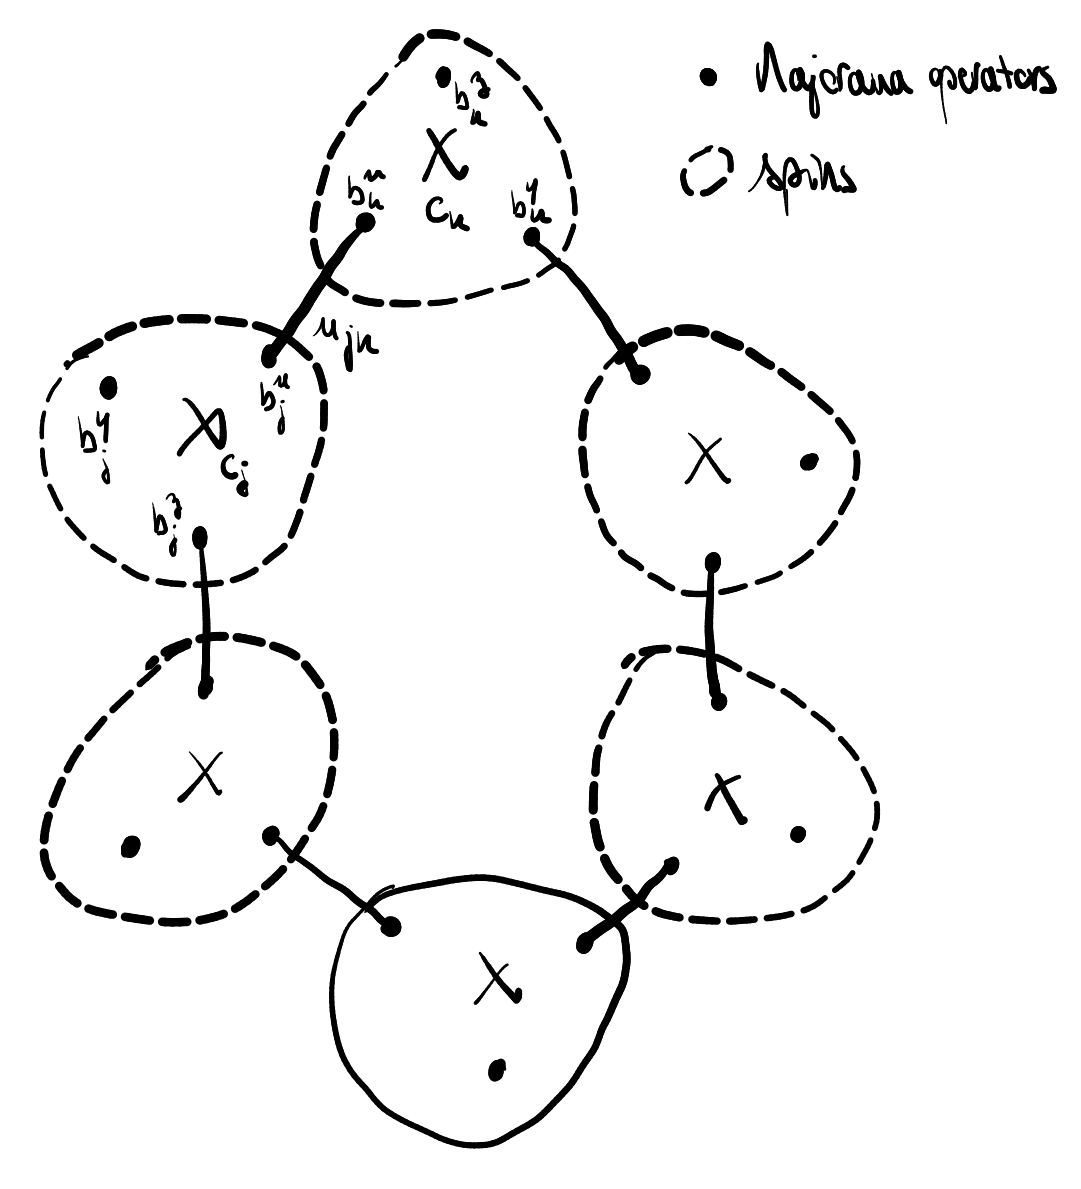
\includegraphics[scale=0.25]{graphs/labelKitaevHCL.png}
            \caption{Representation of the Hamiltonian of the Kitaev model on the Honeycomb lattice with Majorana operators.}
            \label{fig:labelKitaevHCL}
        \end{figure}

		To find the eigenstates of the Hamiltonian, divide the total Hilbert space $\mc L$ into sectors --- eigenspaces of $W_p$ --- which are invariant subspaces of $\mc H$
		\be \mc L = \bigoplus_{w_1,\dotsc, w_m} \mc L_{w_1,\dotsc, w_m} \ee
		with $m$ the number of plaquettes and $w_p = \pm 1$ the eigenvalues of $W_p$, hence remains to solve in a particular sector $\mc L_{w_1,\dotsc, w_m}$. Writing as $n$ the number of vertices, there is approximately $\frac 1 2$ plaquette per vertex, thus $n=2m$, and the dimension of each sector $\mc L_{w_1,\dotsc, w_m}$ is $2^{\frac n 2}$. It can be seen that the degrees of freedom within each sector can be described by Majorana fermions, writing the restricted Hamiltonian as a quadratic form in Majorana operators.

	\section{Spins as Majorana operators}

		Usual systems are described by fermionic operators $a_k$, $k=1,\dotsc, n$, also called fermionic modes. Here introduce the Majorana operators
		\be c_{2k-1} = a_k + a_k^\dagger \qq{and} c_{2k} = \frac{a_k - a_k^\dagger}{i} \ee
		which have the following properties. They are obviously hermitian
		\be c_j^\dagger = c_j \ee
		They anticommute by anticommutation relations
		\be \{c_j,c_l\} = 0 \qq{if} i\neq j \ee
		since for $j = 2k$, remembering only one fermion per state is allowed
		\be \begin{split} c_{2k-1}c_{2k} &= \frac{1}{i}[\cancel{a_j^2} - \cancel{(a_j^\dagger)^2} - a_j a_j^\dagger + a_j^\dagger a_j] \\ &= -\frac 1 i [-\cancel{a_j^2} + \cancel{(a_j^\dagger)^2} - a_j^\dagger a_j + a_j a_j^\dagger ] \\ &= - c_{2k} c_{2k-1} \end{split} \ee
		and for $\abs{j-l} \geq 2$ the anticommutation is straightforward. Finally, easily computed with the same remarks as before
		\be c_j^2 = 1 \label{eq:csquared1} \ee
		all with $j=1,\dotsc, 2n$. 

		Then represent a spin by two fermionic modes, thus by four Majorana operators $b^x,\ b^y,\ b^z, \ c$ instead of $c_1,\ c_2, \ c_3,\ c_4$. They act on a $4$-dimensional Fock space $\widetilde{\mc M}$ when the usual Hilbert space for a spin-$\frac 1 2$ is $2$-dimensional $\mc M \subset \widetilde{\mc M}$. With the operator
		\be D = b^x b^y b^z c : \widetilde{\mc M} \to \widetilde{\mc M} \ee
		the restriction to $\mc M$ is defined as
		\be \ket \xi \in \mc M \iff D \ket \xi = \ket \xi \ee
		$\widetilde{\mc M}$ is denoted as the extended subspace, and $\mc M$ the physical subspace. Hence, $D$ can be thought as a gauge transformation for the group $\mathbb Z_2$. The operator $D$ satisfies the hermiticity
		\be \begin{split} D^\dagger &= c_4 c_3 c_2 c_1 = (-1)^2 c_3 c_4 c_1 c_2 \\ &= (-1)^6 c_1 c_2 c_3 c_4 = D \end{split} \ee
		and the action of a projector
		\be \begin{split} D^2 &= c_1 c_2 c_3 c_4 c_1 c_2 c_3 c_4 = (-1)^3 c_1^2 c_2 c_3 c_4 c_2 c_3 c_4 \\ &= (-1)^6 c_1^2 c_2^2 c_3^2 c_4^2 = 1 \end{split} \label{eq:Dsquared1} \ee
		where in the last equality \eqref{eq:csquared1} has been used.

		The Pauli operators can then be extended to their action on the extended space $\widetilde \sigma^x, \widetilde \sigma^y, \widetilde \sigma^z$, still preserving the physical $\mc M$ by satisfying the same relations as $\sigma^x, \sigma^y, \sigma^z$ when restricted to $\mc M$. The extension goes as
		\be \widetilde \sigma^\alpha = ib^\alpha c : \widetilde{\mc M} \to \widetilde{\mc M} \ee
		for $\alpha=x,y,z$. They indeed satisfy
		\be [D, \widetilde \sigma^\alpha] = 0 \quad (\widetilde \sigma^\alpha)^\dagger = \widetilde \sigma^\alpha \quad (\widetilde \sigma^\alpha)^2 = 1 \quad \forall \alpha \ee
		which can be easily verified, and the relation
		\be \widetilde \sigma^\mu \widetilde \sigma^\nu = \delta^{\mu \nu} + i \varepsilon^{\mu \nu\rho} D \ee
		which is consistent with the fact that $D|_{\mc M} = 1$ giving the expected SU$(2)$ commutation relations for Pauli matrices on the physical $\mc M$. This can be derived as for instance, since \eqref{eq:Dsquared1} and \eqref{eq:csquared1}
		\be \begin{split} \widetilde \sigma^x \widetilde \sigma^y &= i^2 b^x c b^y c = - i^2b^x b^y D^2 \\ &= i^2 b^x b^x b^y b^y b^z c D = i \widetilde \sigma^z D \end{split} \ee
		Considering now many spins each described by four Majorana operators, the Hilbert space goes as
		\be \widetilde{\mc L} = \bigotimes_{j=1}^n \widetilde{\mc M}_j \ee
		with the physical subspace $\mc L \subset \widetilde{\mc L}$, and the operators take the form
		\be \widetilde \sigma^\alpha_j = i b_j^\alpha c \quad D_j = b_j^x b_j^y b_j^z c \ee
		and the restriction still has the same property
		\be \ket \xi \in \mc L \iff D_j \ket \xi = \ket \xi \quad \forall j \ee
		All the relations derived still hold. So the spin Hamiltonian $\mc H\{\sigma^\alpha_j\}$ can be replaced by the fermionic one $\widetilde{\mc H}\{b^\alpha_j,c_j\}=\mc H\{\widetilde \sigma^\alpha_j\}$ restricted to the physical subspace. One can write
		\be \begin{split} \widetilde{\mc H} = &-J_x \sum_{x\text{-links}} (ib_j^x c_j)(ib_k^x c_k) - J_y \sum_{y\text{-links}} (ib_j^y c_j)(ib_k^y c_k) \\ &- J_z \sum_{z\text{-links}} (ib_j^z c_j)(ib_k^z c_k) \end{split} \ee
		It is therefore convenient to introduce the link operators
		\be \hat u_{jk} = ib_j^\alpha b_k^\alpha \ee
		and noting that the index $\alpha$ depends on the direction of the thus $\alpha = \alpha_{jk}$, rewrite
		\be \widetilde{\mc H} = \frac i 4 \sum_{j,k} \hat A_{jk} c_j c_k \label{eq:hamquad} \ee
		with
		\be \hat A_{jk} = \begin{cases} 2 J_{\alpha_{jk}} \hat u_{jk} & \text{if } j \text{ and } k \text{ form a link} \\ 0 & \text{otherwise} \end{cases} \ee
		Note that
		\be \hat u_{jk}^\dagger = \hat u_{jk} \quad \hat u_{jk}^2 =1 \quad \hat u_{jk} = -\hat u_{kj} \ee
		It can be shown easily that
		\be [\hat u_{jk}, \hat u_{lm}] = 0 \quad [\widetilde{\mc H}, \hat u_{jk}] = 0 \quad \forall (j,k), (l,m) \ee
		Indeed
		\be \begin{split} \hat u_{jk}\hat u_{lm} &= i^2 b_j^{\alpha_{jk}} b_k^{\alpha_{jk}} b_l^{\alpha_{lm}}b_m^{\alpha_{lm}} \\ &= (-1)^4 i^2  b_l^{\alpha_{lm}}b_m^{\alpha_{lm}} b_j^{\alpha_{jk}} b_k^{\alpha_{jk}} = \hat u_{lm} \hat u_{jk} \end{split} \ee
		and the commutation with $\widetilde{\mc H}$ follows directly from the commutation between these operators and the fact that there are always two $c_j$ operators in $\widetilde{\mc H}$ cancel the change in sign as
		\be c_jc_k \hat u_{lm} = (-1)^2 \hat u_{lm} c_j c_k \ee
		Hence, the Hilbert space $\widetilde{\mc L}$ split into eigenspaces of $\hat u_{jk}$ index by their corresponding eigenvalues $u_{jk} = \pm 1$ --- notice the removal of the hat for the eigenvalues. Therefore write
		\be \widetilde{\mc L} = \bigoplus_u \widetilde{\mc L}_u \ee
		where the $u$ denotes the collections of all $u_{jk}$ and the sector $\widetilde{\mc L}_u$ has dimension $2^n$ now. Henceforth, the restriction of $\widetilde{\mc H}$ to $\widetilde{\mc L}_u$ is obtained by removing the hats of $\hat u_{jk}$. This allows to write
		\be \widetilde{\mc H}_u = \frac i 4 \sum_{j,k} A_{jk} c_j c_k \label{eq:Hwidetildequad} \ee
		which corresponds to free fermions, and then found the ground state $\ket{\widetilde{\psi}_u}$ exactly.

		It is remarkable to see that
		\be [\widetilde{\mc H}, D_j]= 0 \ee
		Thus, $D_j$ can be seen as gauge transformation of the system, since $\widetilde{\mc H}$ is invariant under $D_j$. The subspace $\widetilde{\mc L}_u$ is not gauge invariant. Indeed the gauge transformation acts as
		\be u_{lm} \to D_j u_{lm} D_j^\dagger = \begin{cases} -u_{lm} & \text{if } l=j \text{ or } m=j \\ u_{lm} & \text{otherwise} \end{cases} \ee
		since $D_j^\dagger D_j = 1$. This is easily seen by performing the same computations as done before making use of the anticommutation relations. Then $D_j$ change the values of $u_{jk}$ on the links connecting the vertex $j$ with the three adjacent vertices $k$. Thus the state $\ket{\widetilde{\psi}_u}$ does not belong to the physical subspace. To obtain the physical ground state, symmetrize over all gauge transformations
		\be \ket{\psi_w} = \prod_j \frac{1+D_j}{2} \ket{\widetilde{\psi}_u} \in \mc L \ee
		where $w$ denotes the equivalence class of $u$ under the gauge transformation. To see this, $w$ is characterized by $w_p = \pm 1$ defined as, choosing a particular direction around the boundary
		\be w_p = \prod_{(j,k) \in \partial p} u_{jk} \ee
		with $j$ in the even sublattice and $k$ the odd one. Also, $w_p$ is invariant under gauge transformation. Thus, the operators
		\be \widetilde W_p = \prod \hat u_{jk} \ee
		commute with the gauge transformation and the Hamiltonian, and the restriction to the physical subspace coincides with the $W_p$. The variables $u_{jk}$ can be seen as a $\mathbb Z_2$ gauge field and $w_p$ the magnetic flux through the plaquette $p$.

	\section{Free fermions Hamiltonian}

		The goal is to write the Hamiltonian in a quadratic form in terms of the fermionic operators. Recall the general form \eqref{eq:Hwidetildequad}
		\be \mc H = \frac i 4 \sum_{j,k} A_{jk} c_j c_k = c^\top A c \ee
		with $A$ a real antisymmetric $n\times n$ matrix, still $n=2m$. The Hamiltonian one seeks for is
		\be \mc H_\text{ff} = \sum_{k=1}^m \varepsilon_k\left( a_k^\dagger a_k -\frac 1 2 \right) \quad \varepsilon_k \geq 0 \ee
		The ground state of such Hamiltonian is thus given by the condition $a_k \ket \psi = 0$, $\forall k$.
		Notice that for $A$ real antisymmetric, there exists $Q\in O(2m)$ such that
		\be A = Q S Q^\top \qq{with} S = \pmqty{0 &  \varepsilon_1 & & & \\ - \varepsilon_1 & 0 & & & \\ & & \ddots & & \\ & & & 0 & \varepsilon_m \\ & & & -\varepsilon_m & 0} \ee
		and the $\{\pm \varepsilon_k\}$ are the spectrum of the Hermitian $iA$. Hence 
		\be c^\top A c =  c^\top Q S Q^\top c = b^\top S b \ee
		with
		\be b_j = \sum_k c_k Q_{kj} \ee
		It can be easily shown that, again by anticommutation relations
		\be \{b_i, b_j \} = 0 \quad b_j^2 = 1 \quad \forall j,k \ee
		Rewriting with the normal modes with a prime
		\be b^\top = (b_1', b_1'',\dotsc, b_m', b_m'') \ee
		and introducing the corresponding ladder operators
		\be a_k = \frac 1 2 (b_k' + ib_k'') \quad a_k^\dagger = \frac 1 2 (b_k' - ib_k'') \ee
		satisfying the relation
		\be \{a_k, b_k^\dagger \} = 1 \ee
		since
		\be \begin{split} a_k a_k^\dagger + a_k^\dagger a_k &= \frac 1 4 ( 2b_k^{\prime 2} + 2b_k^{\prime \prime 2} -ib_k' b_k'' + ib_k'' b_k' + i b_k' b_k'' - ib_k'' b_k') \\ &= \frac 1 4(2 +2) =1 \end{split} \ee
		This finally allows to write 
		\be \mc H = \sum_k \varepsilon_k\left( a_k^\dagger a_k -\frac 1 2 \right) = \frac i 2 \sum_k b_k' b_k'' \varepsilon_k \ee

	\section{Spectrum}

		\begin{figure}[h!]
            \centering
            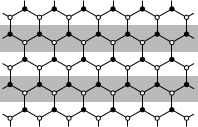
\includegraphics[scale=0.8]{graphs/omegaShaded.png}
            \caption{Part of the lattice --- shaded --- considered for the action of the transformation of interest.}
            \label{fig:omegaShaded}
        \end{figure}

		Take the quadratic Hamiltonian \eqref{eq:hamquad}. Note that the ground state energy does not depend on the signs on the exchange constants $J_{x,y,z}$, since changing the signs can be compensated by changing the corresponding $u_{jk}$. The ground state does not even depend on the signs if $u$ is fixed. To show that, consider for instance $J_z \to -J_z$. This is equivalent to changing $u_{jk}$ for all $z$-links. But the gauge-invariant $w_p$ are constant, thus one can further apply a gauge transformation that make $u_{jk}$ back to its original value. The only effect is that $c_j \to -c_j$. The transformation acts on the shaded area on \autoref{fig:omegaShaded}. So to find the ground and excited states energy, the signs of the exchange constants do not matter.

		\begin{figure}[h!]
            \centering
            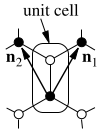
\includegraphics[scale=0.8]{graphs/unitcellhoneylambda.png}
            \caption{Unit cell and the notation used.}
            \label{fig:unitcellhoneylambda}
        \end{figure}

		A theorem by Lieb says that the energy is minimized for $w_p=1$ $\forall p$, thus choose $u_{jk} = 1$ for $j\in$ even and $k\in$ odd sublattice. This configuration has a translational symmetry and thus use Fourier transform to find the spectrum. Represent the site $j$ with $(s,\lambda)$ where $s$ refers to the unit cell and $\lambda$ to the position in the unit cell. The Hamiltonian has then the form
		\be \mc H = \frac i 4 \sum_{s\lambda,t\mu} A_{s\lambda,t\mu} c_{s\lambda} c_{t\mu} \ee
		where the $A_{s\lambda,t\mu}$ dependence is on $\lambda,\mu,t-s$ by translational invariance of the $u_{jk}$. Then write
		\be \widetilde A_{\lambda \mu} (\vb* q) = \sum_t e^{i\vb* q \cdot \vb* r_t} A_{0\lambda,t\mu} \ee
		and 
		\be a_{\vb* q,\lambda} = \frac{1}{\sqrt{2N}} \sum_s e^{-i\vb* q \cdot \vb* r_s} c_{s\lambda} \ee
		The Hamiltonian then becomes, by inverting the relations
		\be \begin{split} \mc H &= \frac{1}{2N} \frac i 4 \sum_{s\lambda,b\mu} \sum_{\vb* q_1} e^{-i\vb* q_1 \cdot \vb* r_b} \widetilde A_{\lambda \mu} (\vb* q_1) \\ &\cdot \sum_{\vb* q_2,\vb* q_3} e^{i\vb* q_2 \cdot \vb* r_s} e^{-i\vb* q_3 \cdot (\vb* r_s + \vb* r_b)} a_{\vb* q_2,\lambda} a_{\vb* q_3,\mu} \\ &= \frac{1}{2N} \frac i 4 \sum_{\lambda,b\mu} \sum_{\vb* q_1} e^{-i\vb* q_1 \cdot \vb* r_b} \widetilde A_{\lambda \mu} (\vb* q_1)  \sum_{\vb* q_4} e^{i\vb* q_4 \cdot \vb* r_b} a_{\vb* q_4,\lambda} a_{-\vb* q_3,\mu} \\ &= \frac i 4 \sum_{\lambda,b\mu} \sum_{\vb* q}  \widetilde A_{\lambda \mu} (\vb* q)  a_{-\vb* q,\lambda} a_{\vb* q,\mu} \\ &= \frac i 4 \sum_{\lambda,b\mu} \sum_{\vb* q}  \widetilde A_{\lambda \mu} (\vb* q)  a^\dagger_{\vb* q,\lambda} a_{\vb* q,\mu} \end{split} \ee
		The spectrum is given by the eigenvalues of $\widetilde A_{\lambda \mu} (\vb* q)$ which is 
		\be  \widetilde A_{\lambda \mu} (\vb* q) = \pmqty{0 & if(\vb* q) \\ -if(\vb* q) & 0} \ee
		with
		\be f(\vb* q) = 2 (J_x e^{i\vb* q \cdot \vb* n_1} + J_y e^{i\vb* q \cdot \vb* n_2}) + J_z) \ee
		and $\vb* n_1,\vb* n_2$ the vectors as in \autoref{fig:unitcellhoneylambda}. Thus
		\be \varepsilon(\vb* q) = \pm \abs{f(\vb* q)} \ee
		Hence, either there exists a $\vb* q$ such that $f(\vb* q)=0$, or there is a gap in the spectrum. Moreover, $f(\vb* q)=0$ has a solution if and only if
		\be \begin{cases} \abs{J_x} \leq \abs{J_y} + \abs{J_z} \\ \abs{J_y} \leq \abs{J_x} + \abs{J_z} \\ \abs{J_z} \leq \abs{J_x} + \abs{J_y} \end{cases} \ee

		The region corresponding is the one that is not shaded in \autoref{fig:triggaphoney}. The 3 gapped phases are distinct but related by rotational symmetry, and there is no continuous transition between two gapped phases.

		\begin{figure}[h!]
            \centering
            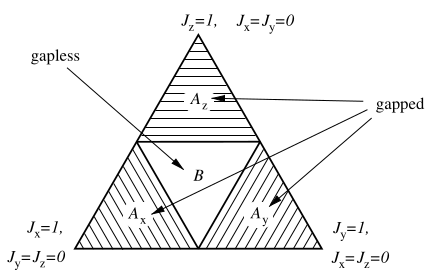
\includegraphics[scale=0.6]{graphs/triggaphoney.png}
            \caption{Phase diagram of the model considered for the spectrum.}
            \label{fig:triggaphoney}
        \end{figure}

		Finally, to relate to quantum spins liquids, the ground state is the superposition of many Majorana modes, thus there is a high level entanglement. Moreover,
		\be \ev{c_j c_k}{\text{GS}} = \delta_{kj} - i B_{kj} \qq{with} B = -i\text{sign}(iA) \ee
		and $A_{kj} = 0$ if $(j,k)$ is not a link, thus $B_{kj}$ too. Hence $\ev{c_j c_k}{\text{GS}} =0$ and there is no long-range interaction, whether or not the system is gapped.

 